\chapterimage{tubes.jpg}

\chapter{Layer 4: Transport}\label{sec:layer4}

\begin{minipage}{0.4\linewidth}
\begin{center}
\begin{bytefield}{16}
\bitbox{16}{Layer 7: Application} \\
\bitbox{16}{\color{color1} Layer 4: Transport} \\
\bitbox{16}{Layer 3: Internet} \\
\bitbox{16}{Layer 2: Network (LAN)} \\
\bitbox{16}{Layer 1: Physical} \\
\end{bytefield}
\end{center}
\end{minipage}
\begin{minipage}{0.6\linewidth}
\begin{center}
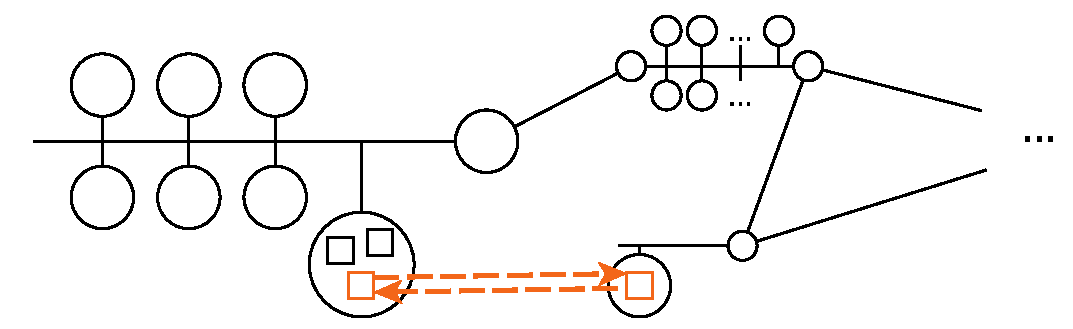
\includegraphics[width=\linewidth]{network_layer4.pdf}
\end{center}
\end{minipage}

\vspace{-0.75cm}

\subsection*{Capabilities}

The \conceptRef{transport}{Transport} layer communicates \conceptRef{process}{processes} (programs)
running in potentially different \conceptRef{host}{hosts}. These processes are identified 
using Layer~4 addresses called \conceptRef{port}{ports}.

The transport layer offers two different ways of communication: without \concept{connections} (\concept{UDP}) 
and with connections (\concept{TCP}~).

\concept{UDP} doesn't establish a \concept{connection} with the destination host because the priority is 
to send some data \concept{payload} as fast as possible. 
Instead, UDP sends packets called \conceptRef{user datagram}{user datagrams} directly to the destination, 
without expecting any sort of confirmation of reception from the destination's UDP layer.
UDP headers are simple and small as well keep the \concept{overhead} of this protocol small.

\concept{TCP} establishes a \concept{connection} before sending any \concept{payload} data
to make sure both ends are ready. In addition, TCP expects \concept{acknowledgment} (confirmation)
of reception of every byte of payload data. Otherwise, data are \conceptRef{retransmission}{retransmitted} 
after a wait period, giving TCP \concept{reliability}. TCP also uses a very clever way 
to limit the data exchange speed (\concept{flow control}) so that fast and slow computers can coexist
and communicate using TCP/IP. To provide all these features, TCP is a more complex protocol than UDP,
uses larger headers and introduces a greater \concept{overhead}.

\begin{exercise}
Which of the following applications do you think use \concept{UDP} and \concept{TCP}?
\begin{itemize}
\item Multiplayer gaming
\item The WWW
\item BitTorrent
\item Video streaming
\end{itemize}
\end{exercise}

\subsection*{Protocols}

\begin{center}
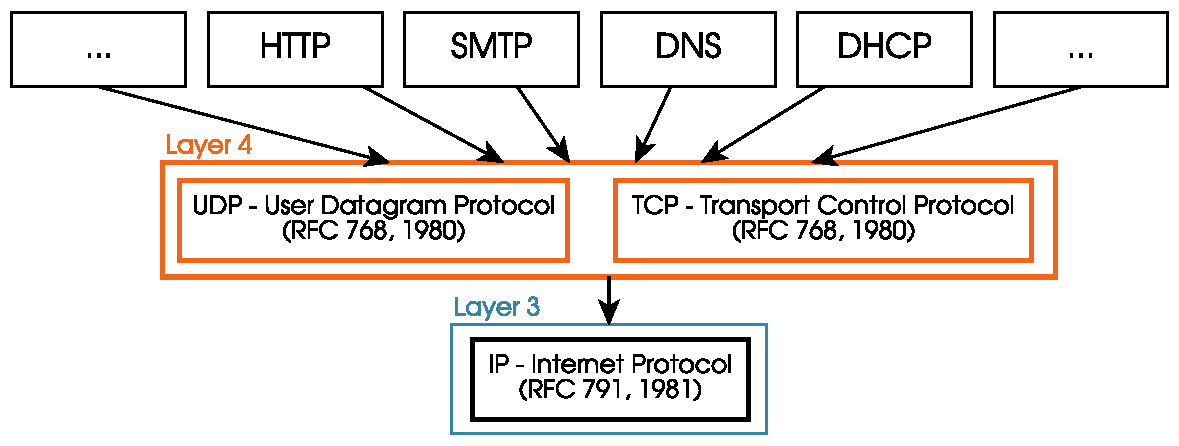
\includegraphics[width=0.95\linewidth]{protocols_layer4.pdf}
\end{center}

The transport layer is at the top of the stack provided by the OS. 
Virtually all applications, and therefore their communication protocols,
employ \concept{TCP}, \concept{UDP} (or even both) to exchange data over the net.
Some important protocols that use TCP or UDP are shown in the previous figure.

Both TCP and UDP encapsulate their PDUs in \concept{IP} \conceptRef{datagram}{datagrams}. 
Generally, \concept{IPv4} is used, but \concept{IPv6} is also a possibility when available.

\begin{remark}
Neither TCP nor UDP change in any way when IPv6 is used instead of IPv4, \ie,
there is not a TCPv6 protocol. Instead, \inlineCode{tcp6} and other expressions that include 
TCP and 6 refer to (regular) TCP over IPv6.
\end{remark}


\section{Layer 4 addressing}

TCP and UDP ``addresses'' are called \conceptRef{port}{ports} and are $16$-bit unsigned integers.
To humans, ports are expressed in two main ways:
\begin{itemize}
\item As a number, \eg, 22, 80 or 443.
\item As the name of the service that typically uses that port, \eg, \concept{sshd}, \conceptRef{HTTP}{http}, \concept{https}.
\end{itemize}

When a Layer~4 PDU is received, the port in its header is used by the OS to know which of the running 
processes must receive the data. 
In turn, processes have to \concept{bind} to a TCP port or to a TCP port (or both)
to let the OS know the port they expect data from.

Only one process may bind to a port at a time for sending data, but TCP and UDP ports
are treated independently:
\begin{itemize}
 \item If a process is bound to port \otherBase{TCP/100}, it will not receive UDP traffic to port 100.
 \item If a process is bound to port \otherBase{TCP/100}, another process (or even the same one) can 
   bind to \otherBase{UDP/100}.  
\end{itemize}

Port number \otherBase{0} is reserved, so the usable range or ports is \otherBase{1}--\otherBase{65535}. 
Ports \otherBase{1}--\otherBase{1023} are only bound to 
processes with1 privileges (\eg, an http \concept{server}), whereas client applications (\eg, an http \concept{client}) 
can only bind to ports \otherBase{1024}--\otherBase{65535} based on their availability.

\begin{exercise}
How many different servers can be run in a machine to provide some feature to other hosts in the network?
\end{exercise}


\section{UDP -- User Datagram Protocol}
\subsection{Packet format}

The \conceptRef{user datagram}{user datagrams} used by UDP all have a $20$-byte header and 
have the following structure:

\begin{center}
\begin{bytefield}{32}
\bitheader{0-31}\\
\bitbox{16}{Source UDP Port} & \bitbox{16}{Destination UDP Port} \\
\bitbox{16}{Length (header and data)} & \bitbox{16}{Checksum} \\
\bitbox[tlr]{32}[bitheight=3em]{Payload data\\{\scriptsize(variable length, byte aligned)}} \\
\bitbox[lbr]{24}{\hspace{3cm}\raisebox{0.25cm}{$\vdots$}} & \bitbox[lt]{8}{} \\
\end{bytefield}
\end{center}

\begin{exercise}\ \\[-0.5cm]
\begin{itemize}
\item What is the maximum payload size that can be sent in a single \concept{user datagram}?
\item Is \concept{fragmentation} desirable when using UDP?
\end{itemize}
\end{exercise}

\subsection{Operation}

\begin{center}
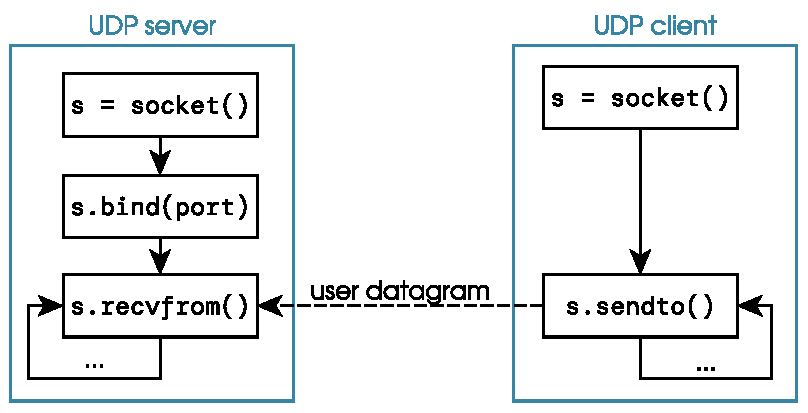
\includegraphics[width=0.5\linewidth]{udp_socket.pdf}
\end{center}

UDP clients first create a \concept{socket} and then directly send the user datagrams with \inlineCode{sendto}.
There is no need to stablish or close a connection.

UDP servers must first \concept{bind} to the port to be exposed to clients, and then 
receive each datagram in an individual call to the read function (\inlineCode{recvfrom}).

The bind function is purely internal to the server: it entails changes in its configuration
(the table mapping port numbers and \conceptRef{process}{processes}), but it does not generate any message. 

\begin{exercise}\ \\[-0.5cm]
\begin{itemize}
\item Can a UDP server work without sending any data through the network?
\item Can a client receive UDP traffic without binding to a port?
\item Can two different hosts bind to the same port and still exchange \conceptRef{user datagram}{user datagrams}?
\end{itemize}
\end{exercise}


\begin{exercise}
The following snippet of code shows a basic UDP server skeleton:

\begin{center}
\showCodeNoOutput{snippets/udpserver.py}
\end{center}

\begin{itemize}
\item Run the server, and in another terminal run \inlineCode{ncat -u localhost 4567} and type some text to test 
  the server.
\item Implement the client end of the communication and test it against the server.
\item What important information do you get if you change \inlineCode{s.recvfrom} to \inlineCode{s.recvmsg}?
\end{itemize}

\begin{remark}
This code uses regular UDP \conceptRef{socket}{sockets}, so it does not need administrator 
nor the \inlineCode{CAP_NET_RAW} capability, as it happened in Exercise~\ref{ex:layer2:echo},
which required access to Layer~2 (\eg, Ethernet) sockets instead.
\end{remark}
\end{exercise}

\section{TCP -- Transport Control Protocol}
\subsection{Packet format}

\concept{TCP} PDUs are called \conceptRef{segment}{segments}. 
Their \concept{header} is at least $20$ bytes long, but can grow longer when certain options are used:

\begin{center}
\begin{bytefield}[bitheight=3em,bitwidth=1.1em]{32}
\bitheader{0-31}\\
\begin{rightwordgroup}{Mandatory\\header part\\{\scriptsize($20$ bytes)}}
\bitbox{16}{Source TCP port} & \bitbox{16}{Destination TCP port} \\
\bitbox{32}{Sequence (seq) number} \\
\bitbox{32}{Acknowledgement (ack) number} \\
\bitheader{0-31}\\
\bitbox{4}{Header\\length/$4$} 
& \bitbox{4}{\otherBase{0}} 
& \bitbox{1}{\rotatebox{90}{\small CWR}} 
& \bitbox{1}{\rotatebox{90}{\small ECE}} 
& \bitbox{1}{\rotatebox{90}{\small URG}} 
& \bitbox{1}{\rotatebox{90}{\small ACK}} 
& \bitbox{1}{\rotatebox{90}{\small PSH}} 
& \bitbox{1}{\rotatebox{90}{\small RST}} 
& \bitbox{1}{\rotatebox{90}{\small SYN}} 
& \bitbox{1}{\rotatebox{90}{\small FIN}} 
& \bitbox{16}{Window size\\{\small (bytes)}}\\
\bitbox{16}{Checksum} & \bitbox{16}{Urgent pointer}
\end{rightwordgroup} \\
\begin{rightwordgroup}[curlyshrinkage=10pt]{Optional\\header part\\{\scriptsize($4$ byte words)}}
\bitbox[tlr]{32}{Options\\{\scriptsize(variable length, optional)}} \\
\bitbox[lbr]{24}{\hspace{3cm}\raisebox{0.25cm}{$\vdots$}} & \bitbox{8}{Padding to\\$32$ bits}
\end{rightwordgroup} \\
\begin{rightwordgroup}[curlyshrinkage=10pt]{Payload}
\bitbox[tlr]{32}[bitheight=3em]{Payload data\\{\scriptsize(variable length, byte aligned)}} \\
\bitbox[lbr]{24}{\hspace{3cm}\raisebox{0.25cm}{$\vdots$}} & \bitbox[lt]{8}{}
\end{rightwordgroup}
\end{bytefield}
\end{center}

TCP headers contain eight $1$-bit flags. Of these, four are used to core TCP features addressed in the following
sections. In the order they appear:
\begin{itemize}
\item ACK: \concept{acknowledgement} flag -- ``\textit{my} ack number is valid''
\item RST: \concept{reset} flag -- ``\textit{abort} the connection''
\item SYN: \concept{synchronization} flag -- ``I'm opening \textit{my} end of the connection''
\item FIN: \concept{fin} flag -- ``I won't send any more \textit{payload} data''
\end{itemize}

\begin{exercise}
How can the receiving end know the size of the options and of the payload data?
\end{exercise}

\subsection{Operation}

TCP is a \concept{stateful} protocol. TCP \concept{sockets} transition between 
multiple states during communication. Each end of the communication has its own 
socket with its own state.
% 
Roughly speaking, connections can be classified as ``Connecting'', 
``Connection established'', or ``Closing connection''.
% 
Payload data is only meant to be exchanged while in ``Connection established''.

\begin{center}
 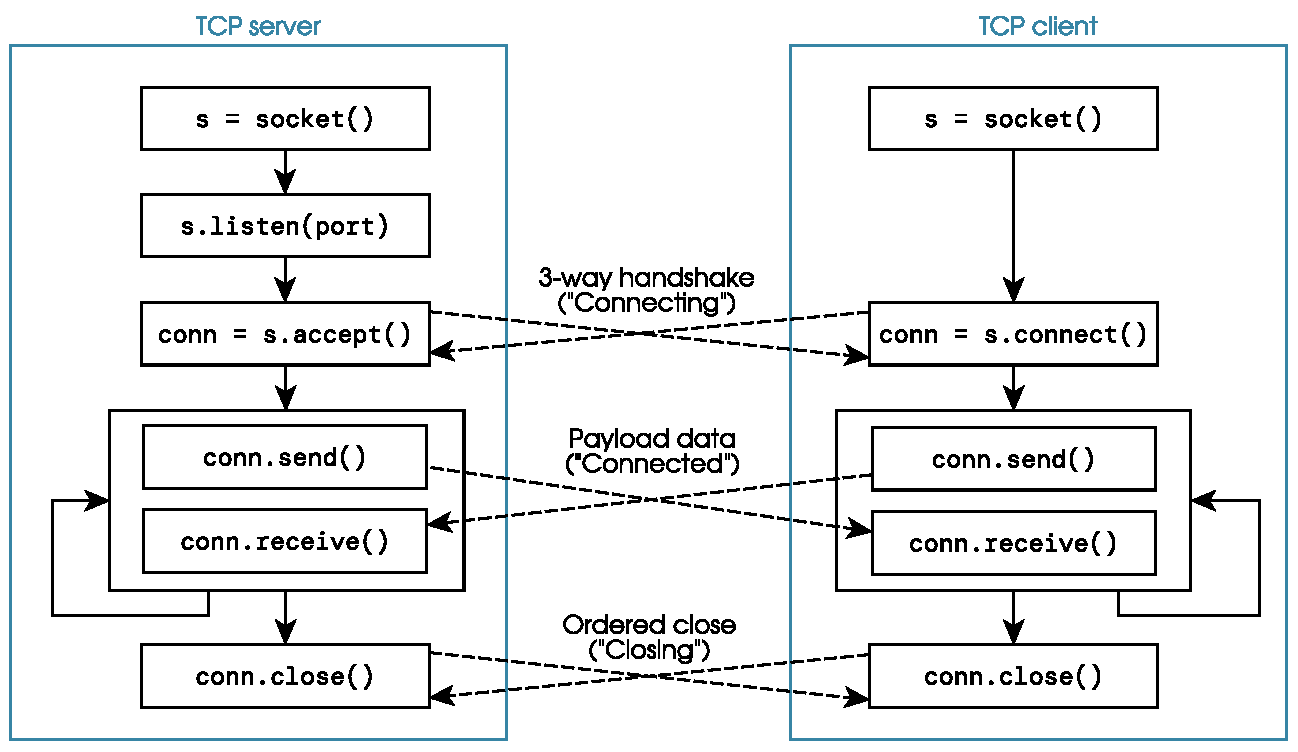
\includegraphics[width=0.75\linewidth]{tcp_socket.pdf}
\end{center}

TCP sockets can be in one of $11$ states. These states, together with two $16$-bit counters 
(\concept{acknowledgement number} and \concept{sequence number}) enable the communication \concept{reliability} 
expected of TCP. The meaning of these states and their transitions are explained in the 
following chapters.

\section{TCP: ``Connecting''}\label{sec:layer4:tcp_opening}

\begin{center}
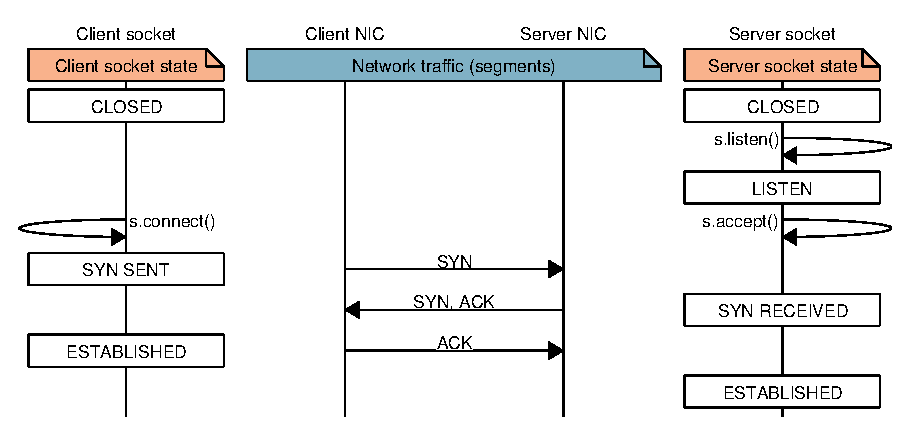
\includegraphics{3_way_handshake.eps}
\end{center}

When a \concept{socket} is created, it beings as \texttt{CLOSED}. 
The end acting as a server begins listening to the service's configured \concept{port}
and changes to the \texttt{LISTEN} state. Payload is not interchanged in this state.

A connection is established via a \concept{3-way handshake} using the 
\texttt{SYN} and \texttt{ACK} header flags.
% 
Each end of the communication reaches the \texttt{ESTABLISHED} state at a different time thanks to 
this handshake. 
Once they do, they are ready to exchange payload data.

\begin{remark}
In TCP, both ends communicate as equal peers, it is unimportant who started the communication. 
That said, normally one end performs an ``active open'' (the client) 
and the other a ``passive open'' (the server).
\end{remark}

Each end of the communication keeps track of its 
\concept{acknowledgement number} (\nack) and \concept{sequence number} (\nseq) counters.
% 
The value of \nseq\ is chosen separately (and typically randomly) by each end: 
$A,\,B \in [0, 2^{32} - 1]$. 

Once during the connection opening, each end sends exactly one segment with the \concept{SYN} flag enabled. 
These segments exchange (synchronize) their initial sequence numbers $A$ and $B$.

Segments with the \concept{ACK} flag enabled (all except for the client's first segment) 
have their \nack\ set to ``the next \nseq\ expected from the other end''. 
This \nack\ should be red as ``I have correctly received all segments corresponding to,
but not including, \nack''. 


The expected \nack\ and \nseq\ numbers during the \concept{3-way handshake} are: 
\begin{center}
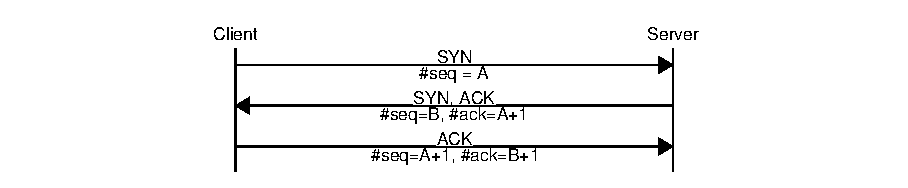
\includegraphics[width=\linewidth]{3_way_handshake_counters.eps}
\end{center}

\begin{exercise}\ \\[-0.5cm]
\begin{itemize}
\item How can one end know that the other end has received their chosen \nseq?
\item Why does the third segment have its \nseq set to $A+1$ and not $A$?
\item What \nseq will the next segment sent by the server have?
\end{itemize}
\end{exercise}


\section{TCP: ``Connection established''}

\subsection{Streams and sequence numbers}

TCP offers the illusion of a data \concept{stream}: two pipes of data in the In and Out directions 
(a \conceptRef{full duplex}{full-duplex} connection). These pipes are \concept{reliable},
\ie, mechanisms are put in place to prevent data loss, duplication and reordering.

\begin{center}
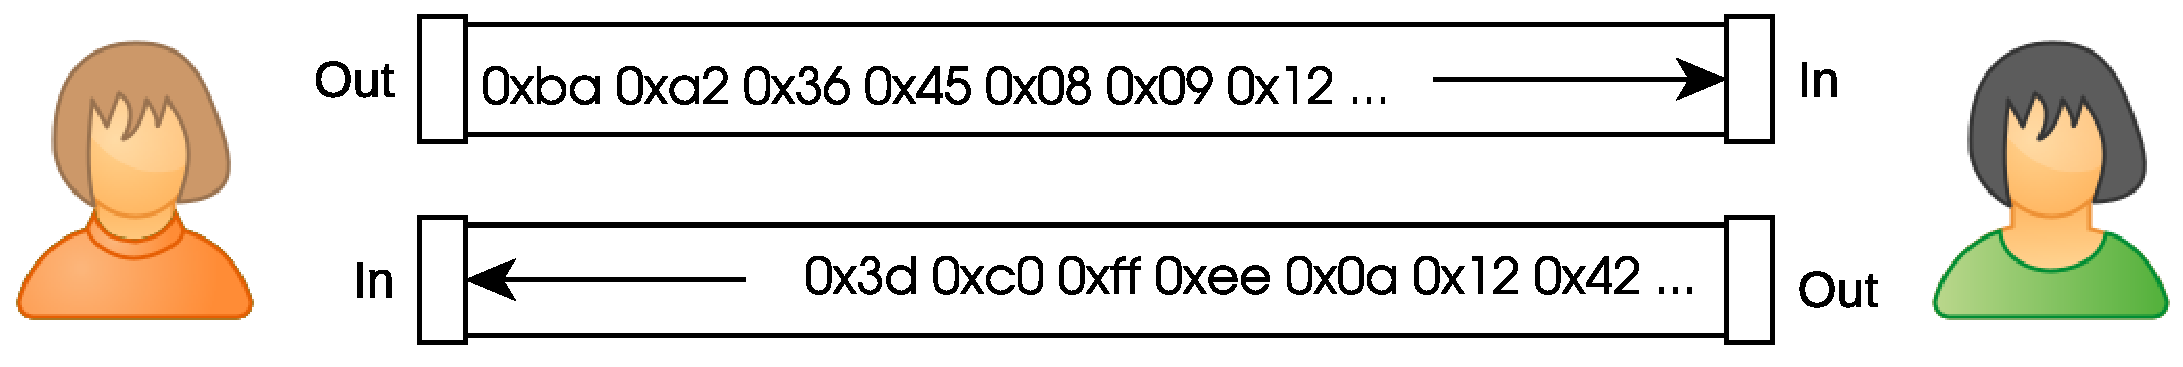
\includegraphics[width=0.75\linewidth]{tcp_two_pipes.pdf}
\end{center}

Every byte of payload data is assigned a sequence number (\nseq) in the TCP header. 
The first byte of payload
data has \nseq\ $=A+1$, where $A$ is the initial sequence number established during connection 
opening (see Section~\ref{sec:layer4:tcp_opening}). Each new byte of data is assigned the next 
\nseq\ (no gaps).

\begin{center}
\begin{tabular}{r |c|c|c|c|c|c|c|c|c|c| l}
\textbf{\nseq} & $A$ & $A+1$ & $A+2$ & $A+3$ & $A+4$ & $A+5$ & $A+6$ & $A+7$ & $A+8$ & $A+9$ & $\cdots$ \\[0.2cm]
\textbf{content}  & \raisebox{-0.5em}{\rotatebox{90}{SYN}} & 
\begin{minipage}{2.5em}
\centering{\otherBase{0x48} \\ \inlineCode{'H'}}
\end{minipage} &  
\begin{minipage}{2.5em}
\centering{\otherBase{0x69} \\ \inlineCode{'i'}}
\end{minipage} &  
\begin{minipage}{2.5em}
\centering{\otherBase{0x21} \\ \inlineCode{'!'}}
\end{minipage} &  
\begin{minipage}{2.5em}
\centering{\otherBase{0x0a} \\ \inlineCode{'\n'}}
\end{minipage} &  
\begin{minipage}{2.5em}
\centering{\otherBase{0x48} \\ \inlineCode{'H'}}
\end{minipage} &  
\begin{minipage}{2.5em}
\centering{\otherBase{0x6f} \\ \inlineCode{'o'}}
\end{minipage} &  
\begin{minipage}{2.5em}
\centering{\otherBase{0x77} \\ \inlineCode{'w'}}
\end{minipage} &  
\begin{minipage}{2.5em}
\centering{\otherBase{0x20} \\ \inlineCode{' '}}
\end{minipage} &  
\begin{minipage}{2.5em}
\centering{\otherBase{0x61} \\ \inlineCode{'a'}}
\end{minipage} &  
$\cdots$ \\
\end{tabular}
\end{center}

\begin{exercise}
The \nseq\ that comes after $2^{32} - 1$ is $0$. Why?
\end{exercise}

Payload data in TCP is always sent together with the \textit{first} position they occupy in the 
\concept{stream} and their length.
For instance, inferring from the data shown above, two segments could be produced:

\begin{enumerate}
\item \nseq\ $= A+1$, len $= 4$, data $= $ \otherBase{0x48 69 21 0a} (\inlineCode{'Hi!\n'})
\item \nseq\ $= A+5$, len $= 13$, data $=$ \otherBase{0x48 6f 77 20 61 72 65 20 79 6f 75 3f 0a}
\end{enumerate}

\begin{exercise}
What would be the \nseq\ of the next segment with new payload data?
\end{exercise}

The receiving end of a TCP \concept{segment} uses this information to stitch together 
a copy the data in the right order, even if the segments themselves arrive out of order. 
%
These data are passed on to the upper \concept{layer} in a 
\conceptRef{buffer}{buffered} fashion, or directly if the \concept{PSH} (push) TCP flag is enabled.

\begin{center}
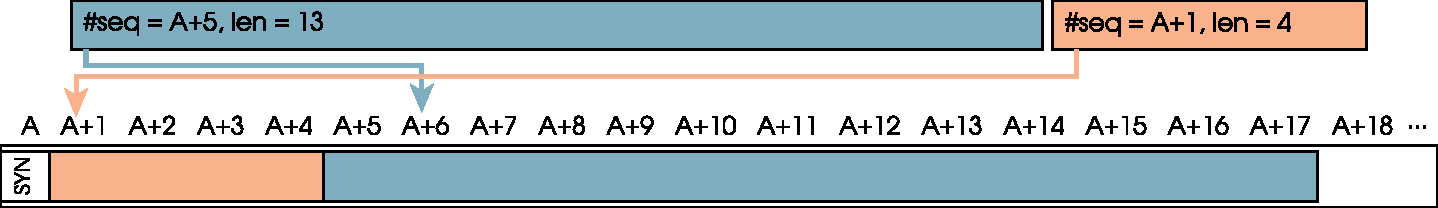
\includegraphics[width=\linewidth]{tcp_reassembly.pdf}
\end{center}


\subsection{Reliability and retransmission}
TCP needs all transmitted data be \conceptRef{acknowledgement}{acknowledged} by the other end.
Whenever some data is received in a TCP segment, the receiving end sends back a confirmation 
even if no data need to be sent at that point.
The acknowledgement number (\nack) in the TCP header is used to tell the other end that all data up to 
(but not including) \nack.

\begin{center}
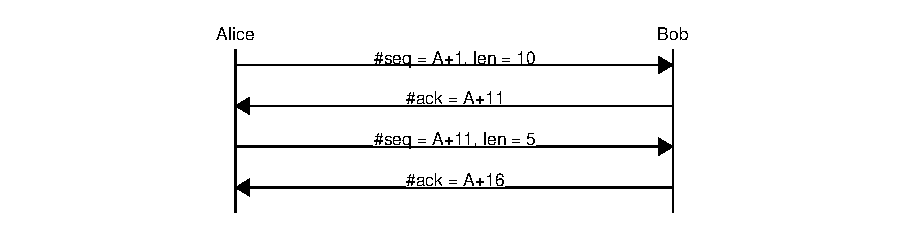
\includegraphics[width=\linewidth]{tcp_ack.eps}
\end{center}

\begin{remark}
The \nseq\ field of a TCP header refers to the sender's sequence numbers. 
The \nack\ field refers to the receiver's sequence numbers.
\end{remark}

Payload data is included in TCP confirmations whenever any data is available.
Conversely, the most recent value of \nack\ is included whenever any data is sent,
\ie, acknowledgments \concept{piggyback} payload data.

For instance, if Alice sends a $50$-byte request, Bob may send his $10$-byte response
and the acknowledgement for Alice's data in the same TCP segment. Alice needs to acknowledge 
Bob's data, and soon sends a segment with no data if needed. Alice will resume sending 
data later when needed.

\begin{center}
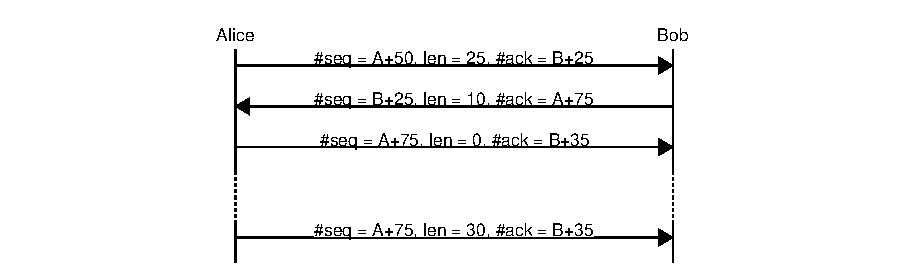
\includegraphics[width=\linewidth]{tcp_ack_piggyback.eps}
\end{center}

A TCP segment that is not acknowledged after a certain wait period is 
\conceptRef{retransmission}{retransmitted}. That time is decided by the OS on each end
based on the average time it takes for a segment to be sent and a reply be received 
(the round-trip time, \concept{RTT}).

Acknowledgements are sent even if that acknowledgement is identical to a previous one. This is because 
acknowledgements can also be lost.

\begin{center}
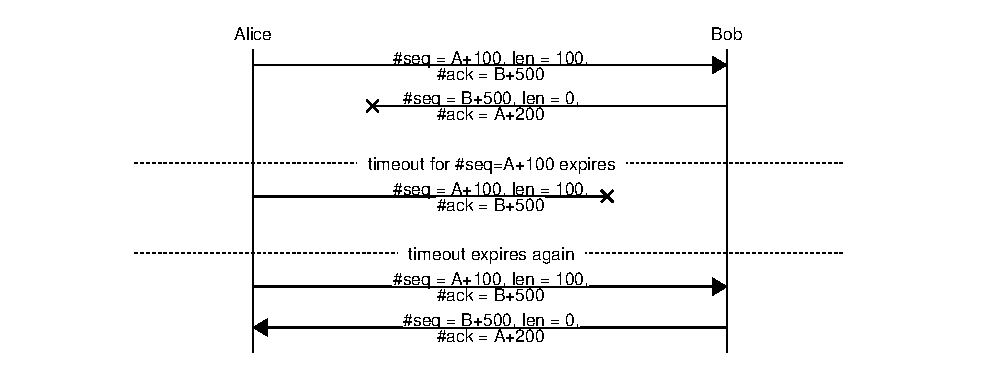
\includegraphics[width=\linewidth]{tcp_ack_retransmission.eps}
\end{center}


\begin{exercise}
Assuming both ends are correctly following TCP:
\begin{itemize}
 \item Provide a set of valid values for (a) to (i).
 \item How does the story change if (f) and (h) are identical/different?
\end{itemize}

\begin{center}
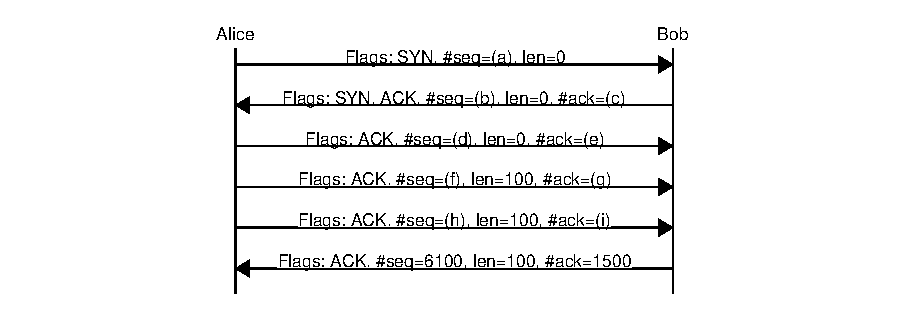
\includegraphics[width=\linewidth]{tcp_ack_exercise.eps}
\end{center}
\end{exercise}

\subsection{Transmission limits}

Data for transmission is often produced in bursts. We would like to send as much 
as possible as soon as possible, but there are two limits put in place in TCP.

The first limit, the \conceptRef{MSS}{Maximum Segment Size (MSS)} is the maximum amount of payload data
per segment allowed in a TCP connexion. 

\begin{center}
\begin{bytefield}[bitheight=3em]{45}
\bitbox{5}{Ethernet header} & 
\bitbox{5}{IP header} & 
\bitbox{5}{TCP header} & 
\bitbox{20}{TCP Payload data}\\[0.25cm]

\bitbox[]{5 }[bitheight=1.5em]{} & 
\bitbox[]{5 }[bitheight=1.5em]{} & 
\bitbox[]{5 }[bitheight=1.5em]{} & 
\bitbox[t]{20}[bitheight=1.5em]{MSS}\\

\bitbox[]{5 }[bitheight=1.5em]{} & 
\bitbox[t]{30}[bitheight=1.5em]{MTU}\\[-0.75cm]
\end{bytefield}
\end{center}

The reason for this limit is to prevent fragmentation, for performance reasons,
\eg, due to the elevated cost in time and memory of reassembly.

The MSS is $536$~bytes in \concept{IPv4} by default,
but can be negotiated with the TCP header Options during the connection opening phase.
In \concept{IPv6}, the default MSS is $1220$~bytes.

\begin{exercise}
Ethernet has an \concept{MTU} of $1500$~bytes. Assuming \conceptRef{datagram}{datagrams} travel 
through 2 Ethernet networks only: 
% 
\begin{itemize}
\item What is the largest \concept{MSS} that cannot cause fragmentation, MSS$_\textrm{max}$?
\item What is the \concept{overhead} for MSS$_\textrm{max}$ and for MSS$_\textrm{max}$ + 1?
\end{itemize}
\end{exercise}

The second limit is to the maximum amount of payload data that can be sent 
before the other end replies with a new \conceptRef{acknowledgement number}{\nack}: 
the so-called \concept{transmission window} size. 
% 
A host will not send data (however much is available, or how urgent it is) until those \nack\ arrive.
% 
When the slower computer replies, it does so always with the most recent \nack.

\begin{exercise}
What is the most likely MSS and transmission window sizes for this example?

\begin{center}
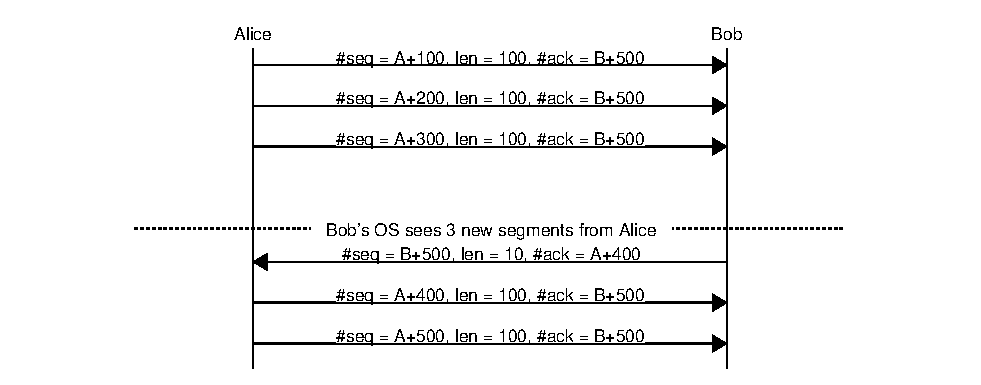
\includegraphics[width=\linewidth]{tcp_ack_window.eps}
\end{center}
\end{exercise}

The value of the transmission window is announced with each and every TCP segment:
this value is a mandatory field of TCP headers.
% 
As the connection progresses, each host can change the value they announce based on 
their own load and necessities.

\begin{remark}
Each host announces its own window size.
\end{remark}


This limit is to prevent fast computers from overwhelming slower (or overworked) ones: 
without the limit the slower computer could need an infinitely increasing buffer size to store the 
not-yet-processed segments sent by the faster computer. With this limit in place, 
at the saturation point, both ends send segments at the same rate even if it takes vastly 
different times to produce and process them.

\section{TCP: ``Closing connection''}\label{sec:layer4:tcp_closing}

\subsection{FIN, \nseq\ and \nack}

Once the connection is \texttt{ESTABLISHED}, it remains so until either end decides to close 
it. 

A node announces it is done sending data and wants to close the connection by sending a 
segment with the \concept{FIN} flag active in the header. The other end may continue 
sending data, in which case it expects replies with updated \nack\ values. The other end 
may also choose to close the connection as soon as it sees the first FIN.
% 
Either way, 
if $k$~bytes of data are sent and $A$
is the initial \nseq, then one segment with \nack\ $= A+k+2$ is expected.

\begin{center}
\begin{tabular}{r |c|c|c|c|c|}
\textbf{\nseq}    & $A$ & $A+1$ & $\cdots$ & $A+k$ & $A+k+1$ \\[0.2cm]
\textbf{content}  & \raisebox{-0.5em}{\rotatebox{90}{SYN}} & Data $\cdots$ & $\cdots$ & $\cdots$ data & \raisebox{-0.5em}{\rotatebox{90}{FIN}} \\[0.2cm]
\end{tabular}
\end{center}

Note how FIN flag occupies a sequence number itself and must be acknowledged like the SYN 
(see Section~\ref{sec:layer4:tcp_opening}), \eg:

\subsection{Two-sided close}

After one end closes its side of the connection, the other may continue sending data indefinitely. 
When the second side is done sending data, it also sends a segment with the \concept{FIN} flag enabled.


\begin{center}
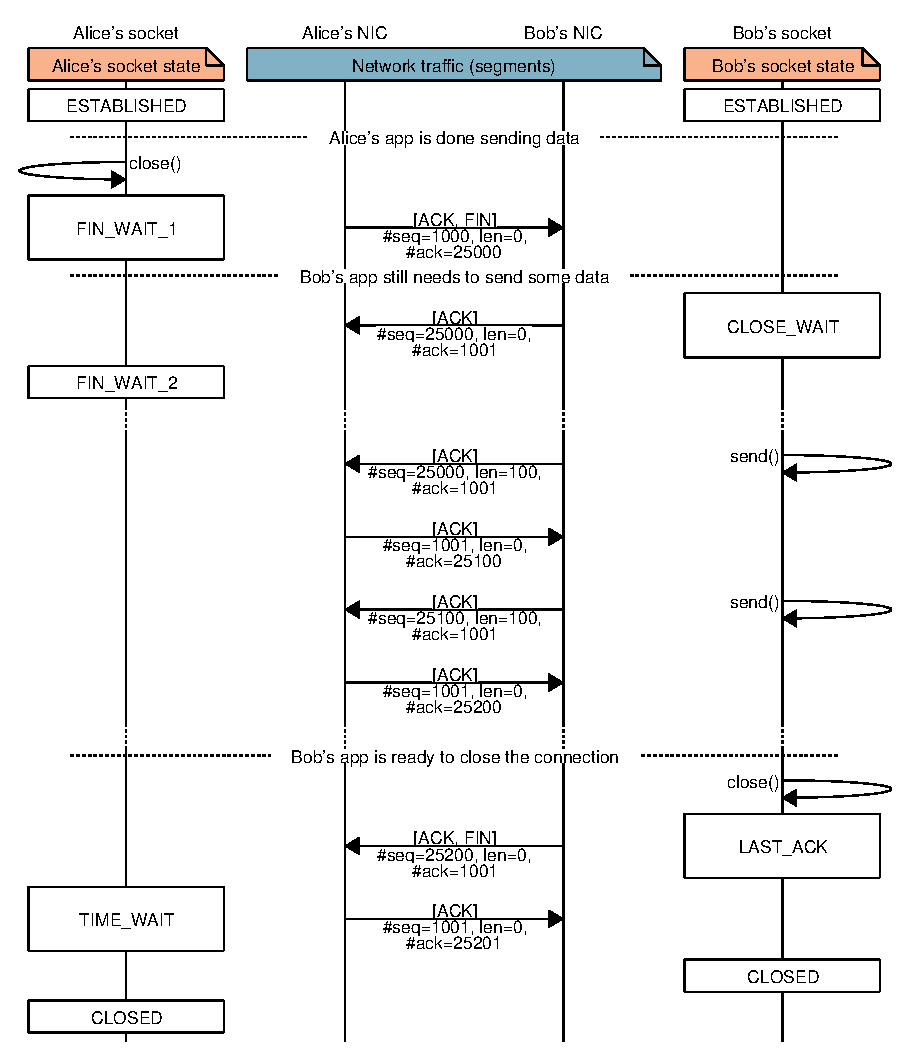
\includegraphics[width=0.9\linewidth]{tcp_close_more_data.eps}
\end{center}

Note that, in case the other end wants to end the connection as it receives a FIN segment,
the closing process is condensed in $3$ instead of $4$ segments, \eg,


\begin{center}
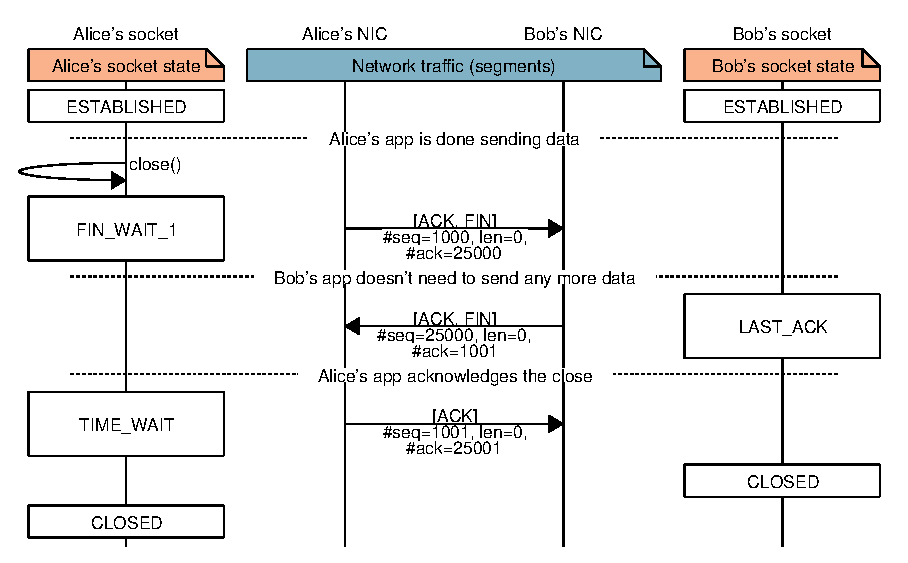
\includegraphics[width=\linewidth]{tcp_close_no_more_data.eps}
\end{center}



\begin{remark}
Note that:
\begin{itemize}
\item Each end sends only one segment with the FIN flag, except for retransmission.
\item The segment with the FIN flag may contain payload data. In that case:
  \begin{itemize}
  \item The payload data occupies sequence numbers \textit{before} the FIN's.
  \item The other end must ACK both the payload data and the FIN.
  \end{itemize}
\end{itemize}
\end{remark}


\subsection{One-sided close}

Sometimes, connections must be terminated and there is not enough time or interest 
to go through the multi-step, two-sided connection closing process.
% 
This may be the case, \eg, when a \concept{process} crashes, a given TCP o UDP port is 
blocked, and other situations of error.

In this scenario, the host that detected the abnormal situation simply sends a segment 
with its \concept{RST} (reset) flag enabled. The receiving ends should not acknowledge
the RST; instead, the connection resources are directly freed, \eg,

\begin{center}
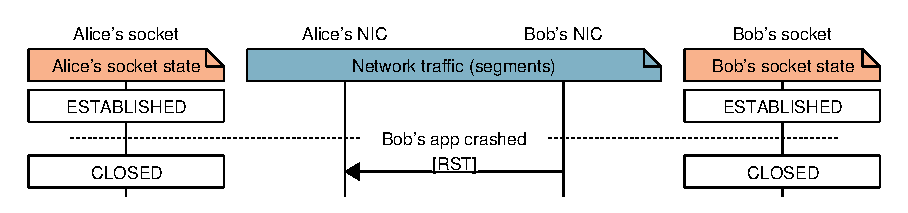
\includegraphics[width=\linewidth]{tcp_close_reset.eps} 
\end{center}

Following the two-sided or the one-sided connection close producedure helps reduce the 
computation resources required to maintain the network stacks of billions of devices worldwide.

\begin{remark}
A connection \textit{cannot} be re-open after it is closed. The RST flag could have been 
more accurately called ``forceful termination''.
\end{remark}

\begin{exercise}
The following diagram displays the $11$ TCP states and (almost) 
all possible state transitions.

\begin{center}
 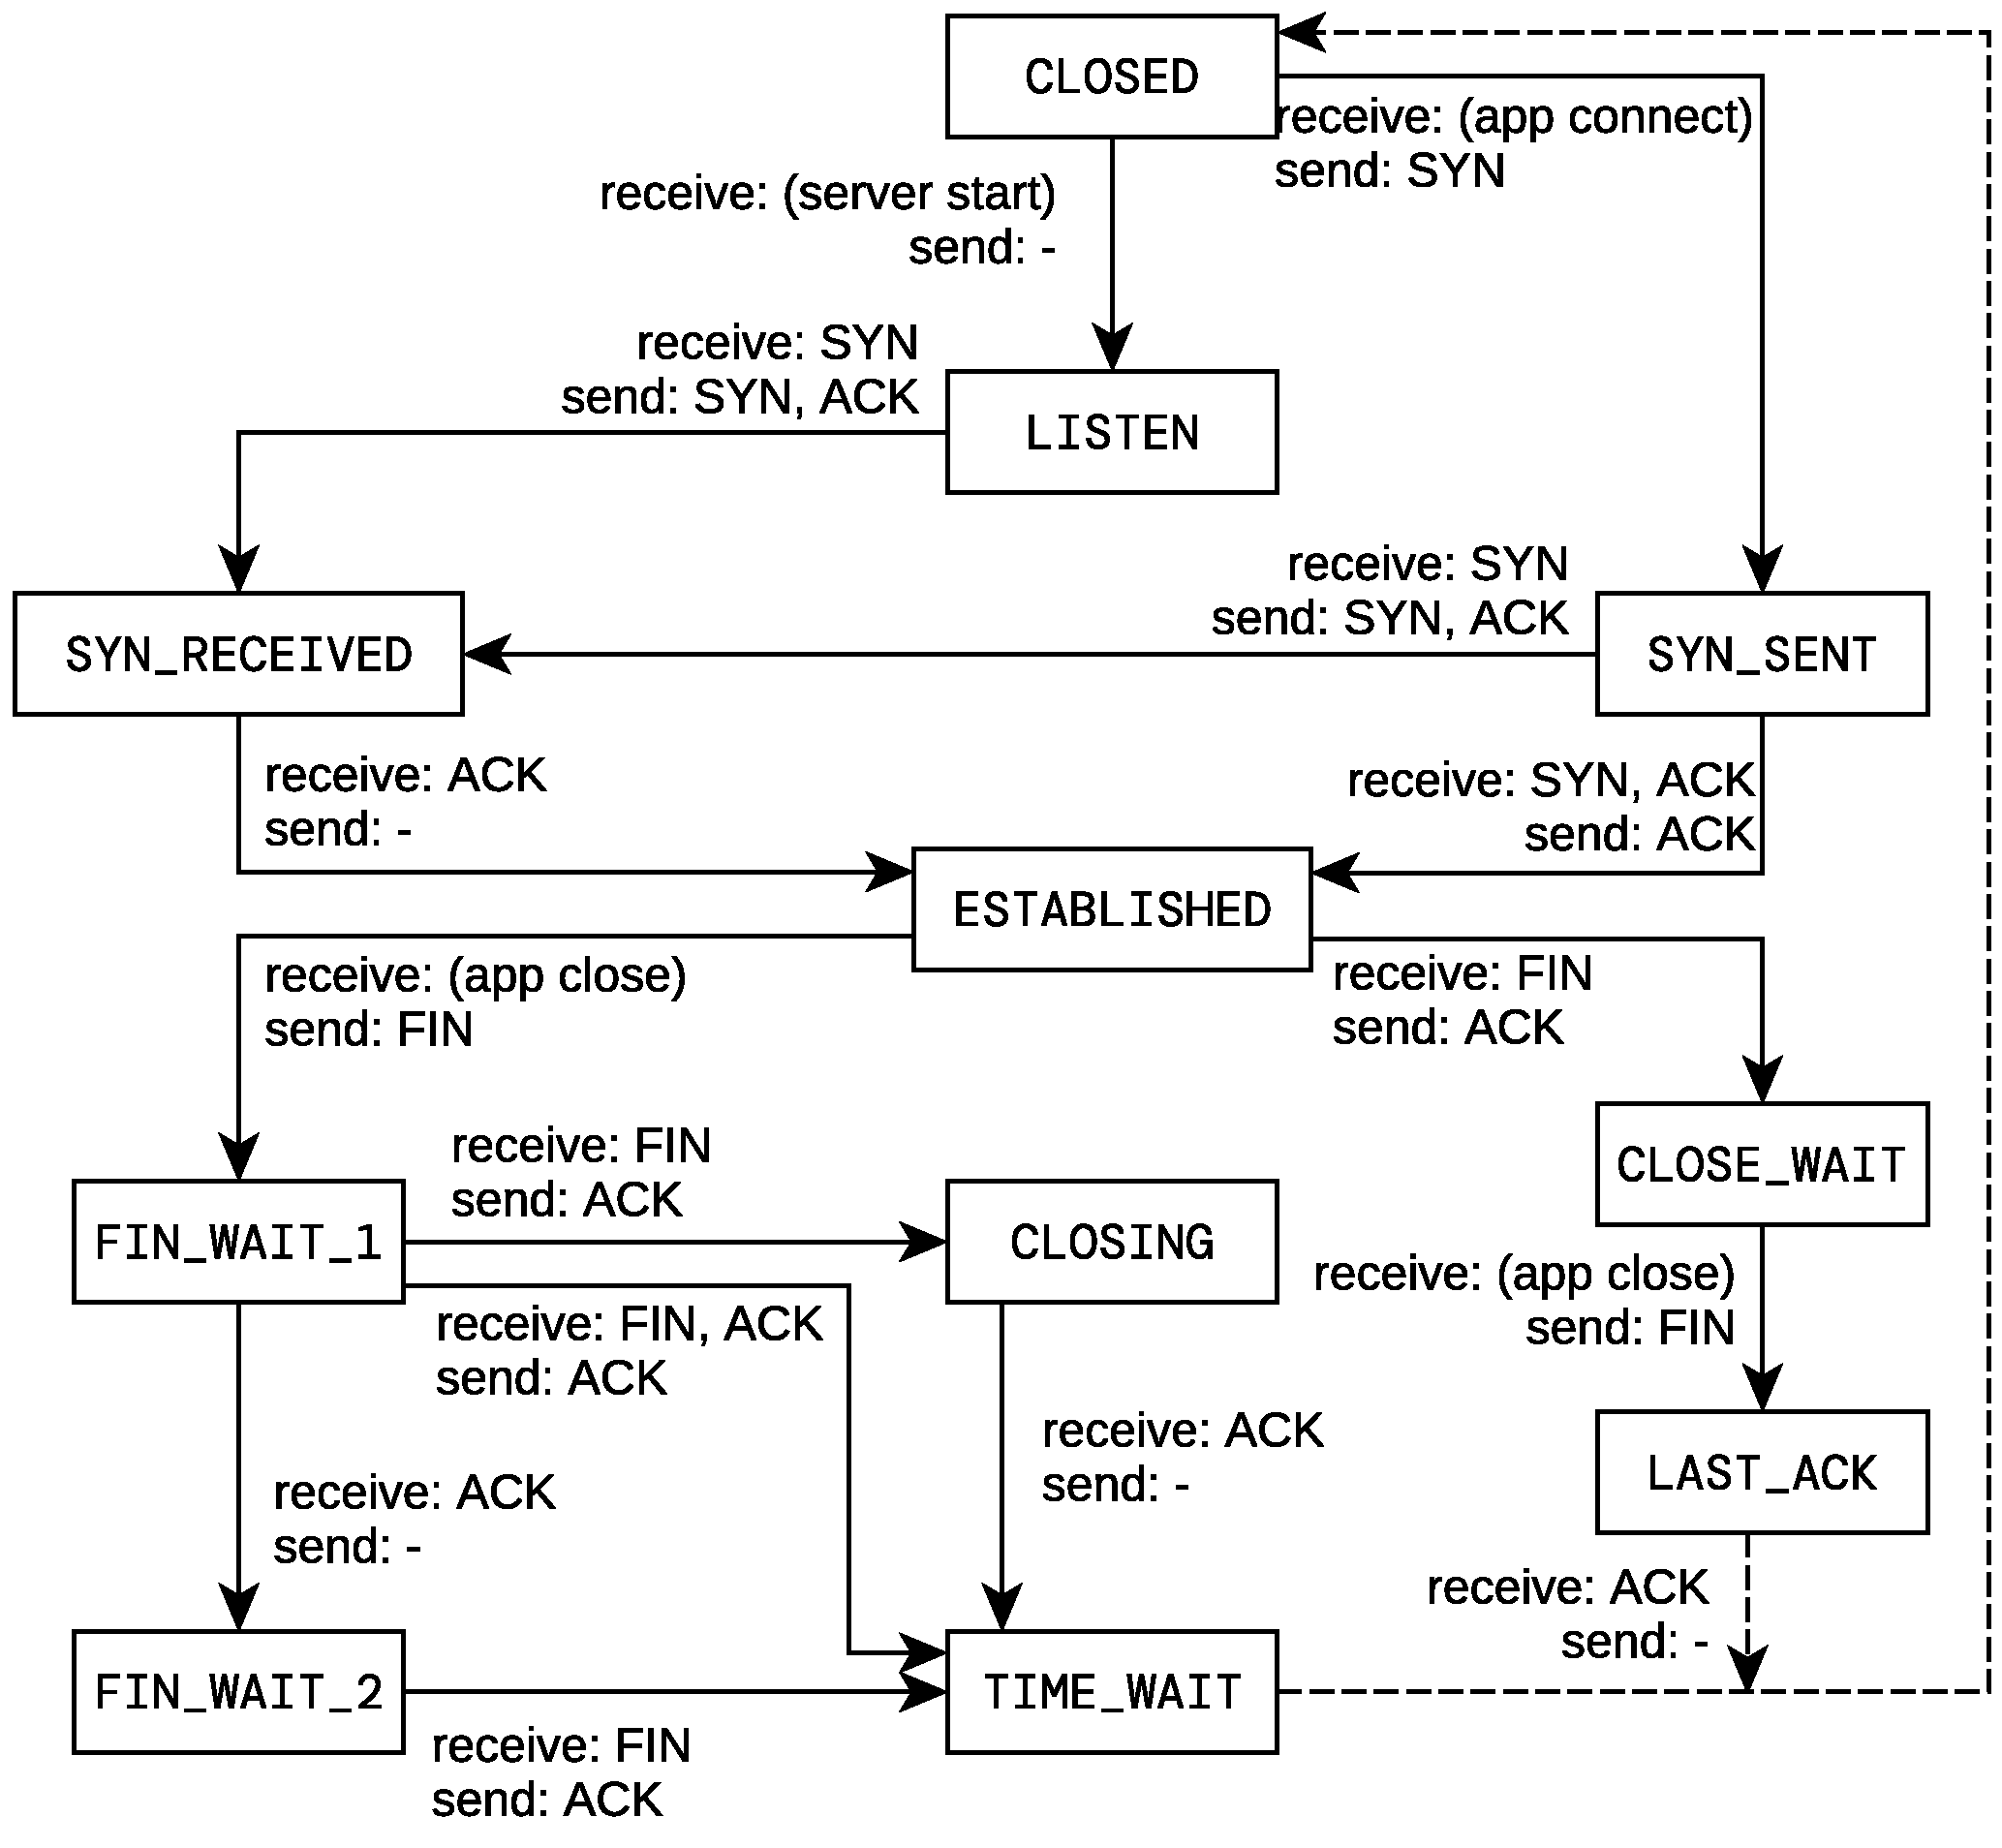
\includegraphics[width=\linewidth]{tcp_state_transition.pdf}
\end{center}

\begin{itemize}
\item Indicate the life cycle of an HTTP server's socket as a path in the graph.
\item Indicate the life cycle of the corresponding HTTP client's socket as a path in the graph.
\item The \inlineCode{CLOSING} state is not described in the previous sections. 
  What do you think is its purpose?
\end{itemize}

\begin{remark}
 This diagram is adapted from ``TCP/IP Illustrated, Volume 2: The Implementation,''
by Gary R. Wright and W. Richard Stevens.
\end{remark}


\end{exercise}
